% XXX Of the next two lines: use first for 1column, second for 2column
%\documentclass[a4paper,12pt,usenames,dvipsnames]{article}
\documentclass[a4paper,10pt,twocolumn,usenames,dvipsnames]{article}

% --- Set up fonts to use ---
\usepackage[bitstream-charter]{mathdesign}
\DeclareSymbolFont{usualmathcal}{OMS}{cmsy}{m}{n}
\DeclareSymbolFontAlphabet{\mathcal}{usualmathcal}
\usepackage{fontspec}
\setmainfont[Scale=0.9, Ligatures=TeX]{Charis SIL}
\defaultfontfeatures[Charis SIL]{Script=latn}
%\usepackage{microtype}                                    % see README
% --- END code for fonts ---
% --- Additional packages here ---
%\usepackage[portuguese]{babel}                             % i18n
%\usepackage{indentfirst}                                   % needed when writing in Portuguese (first paragraph is always indented)
\usepackage{graphicx}
\usepackage{url}                                           % for making urls clickable
\usepackage{epigraph}                                      % for inspirational quotes...
\setlength{\epigraphwidth}{0.8\columnwidth}                % ... with the right length...
\usepackage[font=small,labelfont=bf]{caption}              % proper formatting for caption text
% --- END additional packages ---
% --- Page layout ---
% XXX Of the next two lines: use first for 1column, second for 2column
%\usepackage[top=2.5cm, bottom=2.5cm, left=3.0cm, right=3.0cm]{geometry}
\usepackage[top=2.5cm, bottom=2.5cm, left=1.5cm, right=1.5cm]{geometry}
\setlength{\columnsep}{20pt}
% --- END Page layout ---
% --- Commands (new or redefine) ---
\renewcommand{\footnotesize}{\small}                       % avoid having footnote text too small
% --- END commands ---
% --- Bibliography ---
\usepackage[ % XXX options to be optimised TODO
  style=verbose
 ,backend=bibtex      % biber or bibtex
 ,backref=true
 ,style=numeric-comp  % numerical-compressed
 ,sorting=nyt         % name, year, title
 ,sortcites=true      % some other example options ...
 ,block=none
 ,indexing=false
 ,citereset=none
 ,isbn=true
 ,url=true
 ,doi=true            % prints doi
 ,natbib=true         % if you need natbib functions
]{biblatex} 
% XXX IMPORTANT NOTE XXX: Bibliographic entries that contain a date *MUST* set 
% it in AMERICAN FORMAT: YYYY-MM-DD, otherwise biblatex will IGNORE IT! XXX
% ---
%\addbibresource{pi1.bib}                                   % load bibliography file
% --- END Bibliography ---
% --- HYPER references et al.---
\usepackage{xcolor}                                         % for MidnightBlue colour!
% XXX The hyperref package if used, MUST BE THE LAST ONE included!
\usepackage[pagebackref=false,                             % biblatex takes care of this
            bookmarks=true,
            colorlinks=true,
            linkcolor=MidnightBlue,
            urlcolor=MidnightBlue,
            citecolor=MidnightBlue,
            linktocpage=true]{hyperref}
\hypersetup{pdfencoding=auto}                              % LuaTeX garbles TOC in pdf viewer without this (see: http://tex.stackexchange.com/questions/24445/hyperref-lualatex-and-unicode-bookmarks-issue-garbled-page-numbers-in-ar-for-l)
% --- END HYPER references et al.---
% --- Custom Includes ---
% general purpose
\newcommand{\ts}{\textsection}
\newcommand{\emd}{\textemdash}                             % see [1]

%% prevent figures that end up on the last empty 
%% page of a document from being forcibly centred 
%% on the middle of the page.
\makeatletter
\setlength{\@fptop}{0pt}
\makeatother

% [1] - When inserting an em-dash like this: --- any adjacent words 
%       are NOT HYPHENATED. Using \textemdash (or the newly defined 
%       shortcut)fixes this issue.

% --- math packages (in ArchLinux they're all part of TeXLive) ---

\usepackage{amsmath}   % has to come before eulervm, or things bork!
\usepackage{amsthm}    % required for proof environ (et al.)

% --- END math packages ---

% math stuff
\newcommand{\eqv}{\Leftrightarrow}
\newcommand{\pvec}[1]{\overrightarrow{#1}}
\newcommand{\npvec}[1]{\norm{\pvec{#1}}}
\newcommand{\mb}[1]{\ensuremath \mathbb{#1}}
\newcommand{\mc}[1]{\ensuremath \mathcal{#1}}
\newcommand{\f}[2]{\ensuremath \frac{#1}{#2}}

\providecommand{\abs}[1]{\left \lvert #1 \right \rvert}
\providecommand{\norm}[1]{\left \lVert #1 \right \rVert}

\providecommand{\pth}[1]{\left ( #1 \right ) }
\providecommand{\spth}[1]{\left [ #1 \right ] }
\providecommand{\cpth}[1]{\left { #1 \right } }

% make the optional theorem name bold
\makeatletter
\def\th@plain{%
  \thm@notefont{}% same as heading font
  \itshape % body font
}
\makeatother

% math theorem environments
\newtheorem{thm}{Theorem}[section]
\newtheorem{corollary}[thm]{Corollary}
\newtheorem{lemma}[thm]{Lemma}
\newtheorem{definition}[thm]{Definition} % 'def' cannot be used as environ name

\theoremstyle{remark}
\newtheorem{remark}[thm]{Remark}

\renewcommand\qedsymbol{$\blacksquare$}  % for proofs to end with a black *filled* square (requires amssymb)

%
% math hacks
%

% scalable middle bar; see 
% http://tex.stackexchange.com/questions/5502/how-to-get-a-mid-binary-relation-that-grows
\newcommand{\relmiddle}[1]{\mathrel{}\middle#1\mathrel{}}

% it's a cheat but this makes spacing less wrong around quantifiers
\DeclareMathOperator{\Nexists}{\nexists}
\DeclareMathOperator{\Exists}{\exists}
\DeclareMathOperator{\Forall}{\forall}

% --- END Custom Includes ---
% --- Title page ---
\title{\large\textbf{\huge Skel for \LaTeX}\\
A first sketch for a general template for article writing}
\author{My Name\\\texttt{my.email@provider.tld}}
\date{}
% --- END title page ---
% --- END PREAMBLE ---

\begin{document}
\maketitle                                                 % need full-width title
%\tableofcontents                                           % if needed

\begin{abstract}
  Some tips for a \LaTeX\ template.
\end{abstract}

\section{Styles, et al.}
  Here I'll describe a way of installing \LaTeX\ styles, BiBTeX styles, and a couple 
  of other things in a straightforward way---I think this should work with most 
  *nix systems.

  The first thing to do, is discover where whatever you want to install should 
  be installed. And the ideal way to do this is using a tool named kpsewhich, 
  which should get installed when you install LaTeX. It can be used to do a lot 
  of things (\verb+$ kpsewhich --help+), but the one we’re interested in here, 
  location of styles, uses the \verb+--show-path NAME+ option. The list of 
  allowed names is part of the output of the \verb+--help+ option. So for 
  instance, to discover where to place BiBTeX style files (*.bst), run:
  \begin{verbatim}
kpsewhich --show-path bst
  \end{verbatim}

  This will output a list of locations where BiBTeX style files are searched 
  for. So if you have a file called mystyle.bst, create a folder named 
  ``mystyle" in the appropriate location (I use 
  \verb+/home/user/texmf/bibtex/bst/+), and put mystyle.bst inside the folder 
  you just created. Then run \verb+$ texhash .+ (don’t forget the dot!) from the 
  ``appropriate location'' folder you used. And you're done!

\section{Math Stuff}
  \epigraph{\emph{Ah, the beauty of math!}}{Yours Truly}
  The commands I use for mathematics are included in the file 
  \texttt{custom\_commands.tex}.

  For spacing: In a ``math'' environment, LaTeX ignores the spaces you type and 
  puts in the spacing that it thinks is best. LaTeX formats mathematics the
  way it’s done in mathematics texts. If you want different spacing, LaTeX 
  provides the following four commands for use in math mode: 

  \begin{verbatim}
\; - a thick space

\: – a medium space

\, – a thin space

\! – a negative thin space 
  \end{verbatim}

\section{Graphics}
  % image source: 
  % http://tumblring.net/wp-content/uploads/2011/01/tumblr-tumbeasts.png
  \begin{figure}[ht!]
    \centering
    %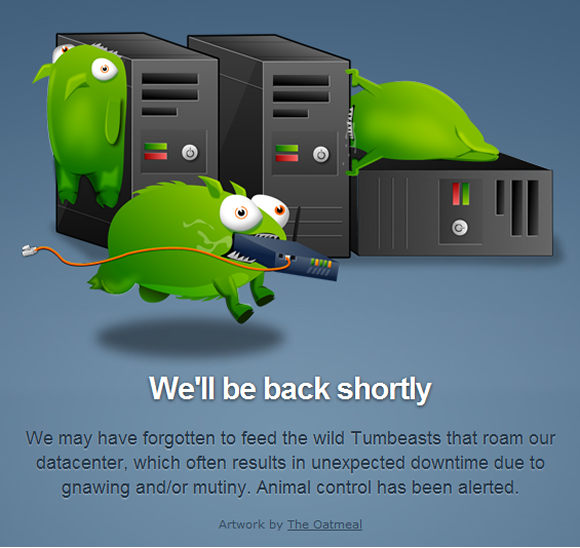
\includegraphics{tumbeasts.jpg}
    %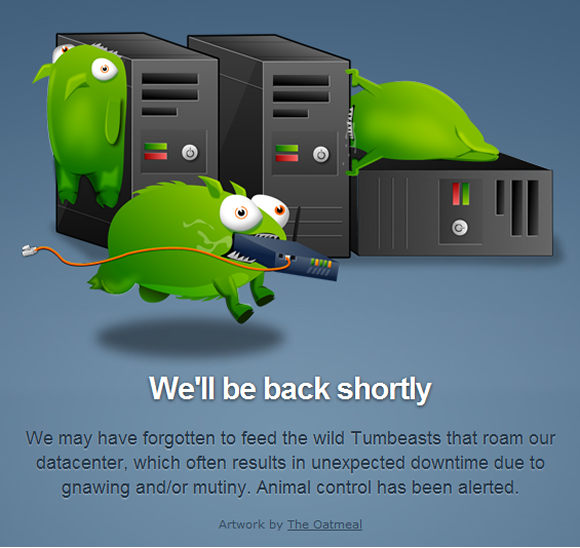
\includegraphics[width=0.5\columnwidth]{tumbeasts.png}
    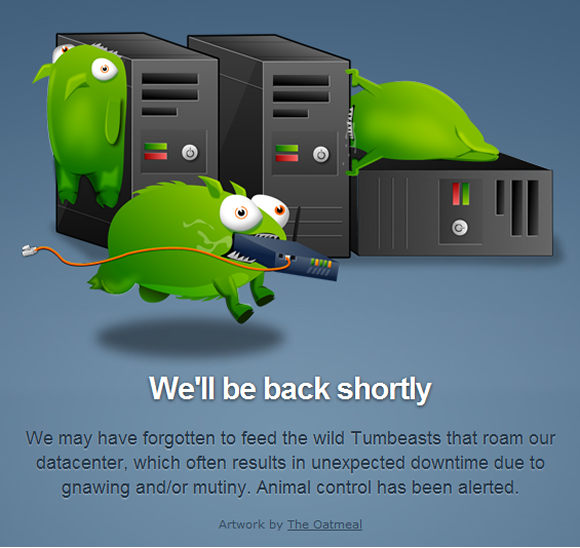
\includegraphics[scale=0.42]{tumbeasts.png}
    \caption{A simple caption}
    \label{overflow}
  \end{figure}

  % for ``articles'' for which you need a custom signature
  % must be used in one-column mode only!
  %\begin{minipage}[c]{\textwidth}
  %  \vspace{1cm}
  %  \flushright\parbox{7.5cm}{\emph{Yours sincerely}\\
  %  \\[1.0cm]
  %  Yours Truly's Full Name}
  %  \flushright\parbox{7.5cm}{}
  %  \vspace{1cm}
  %\end{minipage}

%\printbibliography
\end{document}
